%Incidencia de una onda plana a 45° con n_i = 1, n_t = 1.46   

\documentclass[tikz,crop]{standalone}

\usepackage{tikz}
\usetikzlibrary{decorations.pathreplacing,decorations.pathmorphing}
\usepackage{physics}

\begin{document}


	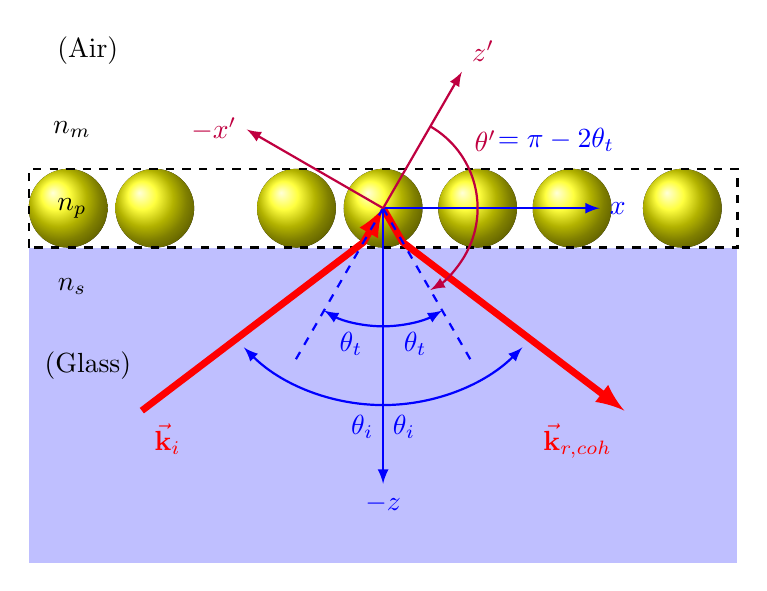
\begin{tikzpicture}[scale=1]
\def\a{.5}
\def\d{.5}

\fill[blue, opacity=.25] (-4.5,-4\d) rectangle (4.5,-\d);

\foreach \x in {-4,-2.9,-1.1,0,1.2,2.4,3.8}{
\fill[ball color=yellow, opacity=1] (\x,0) circle(\a);}


\draw[thick, dashed] (-4.5,-\d) rectangle (4.5,\d);

\draw[latex -, thick, red, line width=2.5](0,0)--(-120:.5)--(-140:4) node[anchor=north west]{$\va{k}_i$};
\draw[- latex, thick, red, line width=2.5](0,0)--(-60:.5)--(-40:4)node[anchor=north east]{$\va{k}_{r,coh}$};

\draw[- latex, thick, blue] (0,0)--(-90:3.5) node[anchor = north]{$-z$};
\draw[- latex, thick, blue] (0,0)--(0:2.75) node[anchor = west]{$x$};

\path (0,0)++(-90:2.5)node[anchor=north east, blue]{$\theta_i$}; 
\draw[- latex, thick, blue](-90:2.5)arc(-90:-45:2.5);
\path (0,0)++(-90:2.5)node[anchor=north west, blue]{$\theta_i$}; 
\draw[- latex, thick, blue](-90:2.5)arc(-90:-135:2.5);

\draw[thick, blue, dashed](0,0) -- (-120:2.25);
\draw[thick, blue, dashed](0,0) -- (-60:2.25);
\path (0,0)++(-90-50/2:1.6)node[anchor=north west, blue]{$\theta_t$}; 
\draw[- latex, thick, blue](-90:1.5)arc(-90:-60:1.5);
\path (0,0)++(-90+50/2:1.6)node[anchor=north east, blue]{$\theta_t$}; 
\draw[- latex, thick, blue](-90:1.5)arc(-90:-120:1.5);

\draw[- latex, thick, purple] (0,0)--(60:2) node[anchor = south west ]{$z'$};
\draw[- latex, thick, purple] (0,0)--(150:2) node[anchor =  east]{$-x'$};
\path (0,0)++(30:1.2)node[anchor=south west, purple]{$\theta'$}; 
\path (0,0)++(30:1.2)node[anchor=south west, blue]{$\;\;\; =  \pi - 2\theta_t$}; 
\draw[- latex, thick, purple](60:1.2)arc(60:-60:1.2);

\node at (-3.75,2) {(Air)};
\node at (-4,1) {$\; n_m$};
\node at (-4,0) {$\; n_p$};
\node at (-4,-1) {$\; n_s$};
\node at (-3.75,-2) {(Glass)};	
\end{tikzpicture}




\end{document}
